\documentclass[12pt, dvipdfmx]{jarticle}
\usepackage{ilsfonts}    % 卒論スタイルで使うフォントの定義
\usepackage{ilssoturon}  % 卒論スタイル宣言
\usepackage[dvips]{graphicx} % グラフィクスの利用宣言
\usepackage{amsmath,amssymb} % 数学記号などの利用宣言
\usepackage{bm}  % 太字数式文字の利用に関する宣言
\numberwithin{equation}{section}
%\usepackage{slashbox} % 表に斜線を入れる(不要かも)
%\usepackage[dvips]{graphicx,psfrag} % 図に数式を使うときに用いる(別の方法がおすすめ)
%\usepackage[dvipdfmx]{graphicx} %図
% ハイパーリンクを作るためのパッケージだが,pdf viewerによってはハイパーリンクの枠が描画
% されたまま出力されるので,基本的には使用しない
%\usepackage[dvipdfmx]{hyperref}
%\usepackage{pxjahyper} % 日本語しおりを作るためのパッケージ
%% 以下は論文表紙に出力される内容
\年度{2024年度}
\提出日{2024年1月xx日}
\研究者{2131007 &安達 拓真}
\論文題目{Artificial Bee Colonyアルゴリズムによる\\サポートベクトルマシン
の\\ハイパーパラメータ最適化}

\begin{document} % ここから論文本体
\卒論表紙 % これで数式が出る

% 以下の4行は目次を定義している
% 正しく目次を出力するためには tex コンパイルを2回連続でかけること
\pagenumbering{roman} % 目次のページ番号はローマ数字
\tableofcontents % 目次を出す命令
\clearpage % 改ページ
\pagenumbering{arabic} % ページ番号をアラビア数字になおす

% ここからが論文本体。ただし、訂正がしやすいように節ごとにファイルを
% 分割している。ここに論文本体を入れてもコンパイルは可能だか、
% けっしておすすめできない。
\section{はじめに}
機械学習モデルには,あらかじめ決めておかなければいけない値であるハイパーパラメータが
存在する.
これらのハイパーパラメータはモデルの性能に大きな影響を与えるため,
適切なハイパーパラメータの選択が必要不可欠である\cite{essential}.
ハイパーパラメータの例として,分類や回帰に用いられるサポートベクトルマシン(SVM)では,
ペナルティパラメータ$C$やカーネル関数のパラメータが挙げられる.
これらのハイパーパラメータは離散、連続、カテゴリなど様々である.
そのため,ハイパーパラメータ最適化(Hyper Parameter Optimization, HPO)
では,高次元かつ複雑な探索空間の探索が必要である.
さらに,目的関数を評価するためにモデルの学
習が必要となるため,
多くの場合目的関数の評価が実行時間におけるボト
ルネックとなる.
そのためHPOでは評価回数と実行時間がトレードオフの関係にある\cite{trade}.

従来のハイパーパラメータ調整は手動調整やグリッドサーチ,ランダムサーチで行われてきた.
手動でハイパーパラメータを調節することは直感と経験に頼る作業になり,
グリッドサーチ,ランダムサーチでは自動化されたものの,
探索効率が悪く,高次元の探索空間では計算コストが大きな課題となる.

これらの課題を解決するため,より効率的な探索手法として,群知能が注目されている.
群知能とは,自然界の生物の群れが高度な振る舞いをすることをコンピュータに適用したアルゴリズムである\cite{population}.
群知能の代表的な手法には,人工蜂コロニー(ABC),粒子群最適化(PSO),蟻コロニー最適化(ACO)
などがある.
特にABCは,設定パラメータが少なく比較的シンプルなアルゴリズムであるため,
HPOの最適化アルゴリズムとして適している.

先行研究では,ABCを用いてSVMのハイパーパラメータ最適化と特徴選択を行い,
SVMのカーネル関数を固定して実験を行っていた\cite{origin}.
しかしSVMには様々なカーネル関数が適用でき,それぞれハイパーパラメータが異なる.
そのため,カーネル関数の選択をハイパーパラメータとして扱うことは,
より良いSVMモデルの探索を可能にする可能性がある.

そこで本研究では,
先行研究で固定されていたカーネル関数を含むハイパーパラメータ全体を探索対象とし,
ABCアルゴリズムを用いてSVMのハイパーパラメータ最適化を行う.
具体的には,$C$,4種類のカーネル関数(線形,RBF,シグモイド,多項式),
およびそのカーネル関数に対応するパラメータを最適化対象とする.
これにより,SVMの分類性能をさらに向上させることを目的とする.
 本研究では,10\%KDD99データセットを使用して提案手法と先行研究との比較実験を行った.
その結果提案手法で得られたパラメータセットは,先行研究で得られたものよりも分類精度が高いという結果となった.
混同行列の評価も書く.
以降の構成は,2章と3章にてSVMとABCの理論を示し,4章で提案手法の説明を行なう.
5章で実験,6章で考察.
 % intro.tex を読み込む。
\clearpage % 改ページ(節が終るごとに改ページしてください)
\section{サポートベクターマシン(SVM)}
SVMは1995年にCortesらによって提案された機械学習アルゴリズムである\cite{svm}.
SVMは教師あり学習を用いる2値分類器であるが,多クラスへの拡張も可能である.
SVMは,訓練サンプル集合からデータを分類する識別関数を学習する.
この学習過程において,SVMは訓練データの中で識別関数に近いデータであるサポートベクターを得る.
そして,サポートベクターと識別関数との距離,すなわちマージンを最大化するように識別関数を構築する.
これにより,SVMは新しいデータを分類する際,
最大限のマージンを持ってデータを分類できるようになり,
未知のデータに対しても誤分類のリスクを最小限に抑えることができる.
\subsection{ハードマージンSVM}
$n$個の$N$次元教師データ$\boldsymbol{x}_i(i=1,...,n)$,
がクラス$K_1$,$K_2$の2値分類データであるとして,
対応するクラスラベルをクラス$K_1$の時に$y_i= 1$,
クラス$K_2$の時に$y_i= -1$とすると,データが線形分離可能であれば
識別関数は(\ref{decision})式のように定義される.
 $\boldsymbol{w}$は$m$次元ベクトル,$b$は識別関数のパラメータである.
\begin{align}
    \label{decision}
f(\boldsymbol{x}) = \boldsymbol{w}^T \boldsymbol{x} + b
\end{align}
すべての教師データ$\boldsymbol{x}_i(i=1,...,n)$について(\ref{learn})式の条件を満たすように
$\boldsymbol{w}$, $b$を調節する事がSVMの学習フェーズとなる.
\begin{align}
    \label{learn}
    f(\boldsymbol{x}) = \boldsymbol{w}^T \boldsymbol{x}_i + b =
    \begin{cases}
        \geq 1&  \boldsymbol{x}_i \in K_1 \\
        \leq  -1& \boldsymbol{x}_i \in K_2
    \end{cases}
\end{align}
このとき,(\ref{learn})式は(\ref{equal})式と等価になる.
\begin{align}
    \label{equal}
    y_i(\boldsymbol{w}^T \boldsymbol{x}_i + b) \geq 1
\end{align}
\begin{figure}
    \centering
    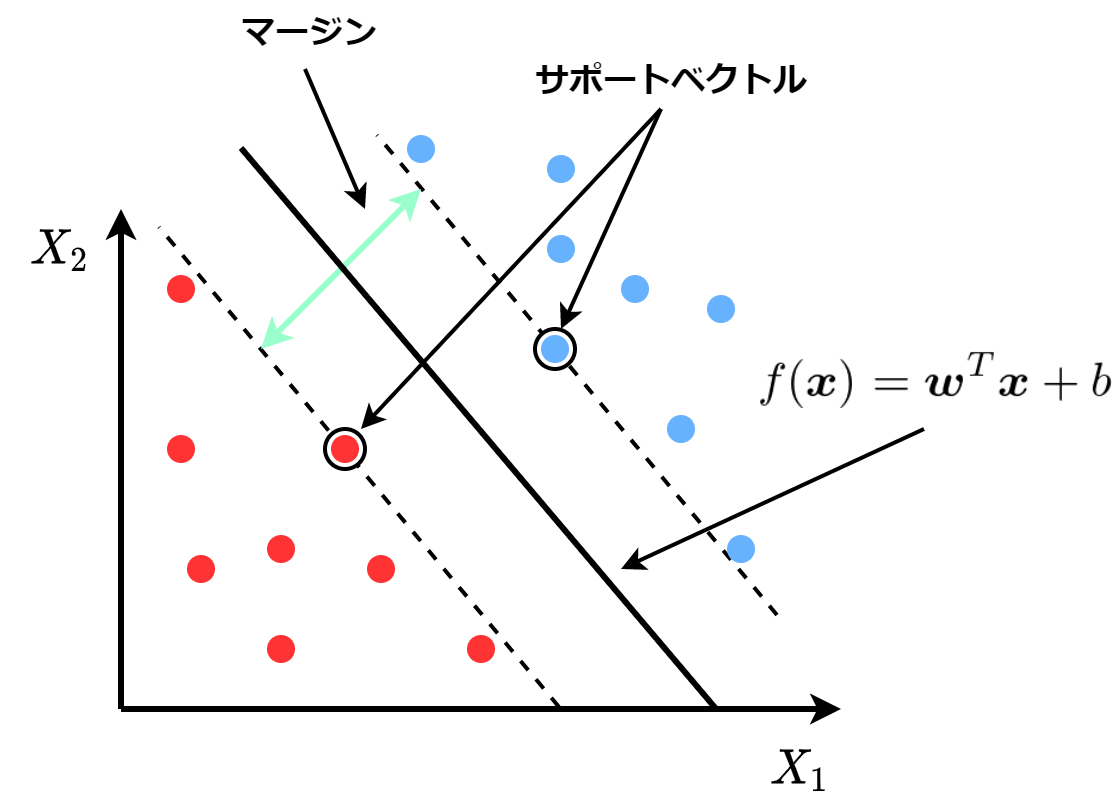
\includegraphics[width=0.6\linewidth]{svm_support.png}
    \caption{SVMの分類方法}
    \label{svm_support}
\end{figure}
ここで図~\ref{svm_support}にデータを分離する超平面(2次元では直線)を示す.
分離超平面とそれに最も近いデータ(サポートベクター)との距離をマージンと呼び,
SVMはマージンを最大化するように分離超平面を求める.
マージンを最大化することで,
サポートベクターから少しずれたデータが存在しても分類可能になり,
モデルの汎化性能が向上する.
次に,マージンを最大化する超平面を求める方法を導く.
$\boldsymbol{x}_i$から超平面への距離を$d$とすると,
$d$は(\ref{distance})式のようになる.
\begin{align}
    \label{distance}
d = \dfrac{|f(\boldsymbol{x_i})|}{\|\boldsymbol{w}\| }
\end{align}
よって,マージンを$M$とすると,
マージン最大化は(\ref{margin})式の最適化問題によって表現できる.
\begin{align}
    \label{margin}
    \underset{{\boldsymbol{w},b}}{\text{max}}~M,~~ \text{subject to } \dfrac{y_i(\boldsymbol{w}^T \boldsymbol{x}_i + b)}{\|\boldsymbol{w}\|}
    \geq M ~~  (i=1,...,n)
\end{align}
さらに,(\ref{margin})式の制約条件部分を$M$で割り,
$\frac{\boldsymbol{w}}{M\|\boldsymbol{w}\|}$と
$\frac{b}{M\|\boldsymbol{w}\|}$
をそれぞれ$\tilde{w}$,$\tilde{b}$
とすると制約条件は(\ref{chmargin})式に書き換えられる.
\begin{align}
    \label{chmargin}
    y_i(\boldsymbol{\tilde{w}}^T \boldsymbol{x}_i + \tilde{b}) \geq 1
\end{align}
(\ref{chmargin})式の等号が成立するデータ
$\boldsymbol{x_i}$は分離超平面と距離が最も近いデータ,
すなわちサポートベクターである.
したがってマージン$\tilde{M}$は(\ref{newmargin})式のようになる.
\begin{align}
    \label{newmargin}
   \tilde{M} = \dfrac{1}{\|\boldsymbol{\tilde{w}}\|}
\end{align}
よって(\ref{margin})式は(\ref{finalmargin})式で表すことができる.
\begin{align}
    \label{finalmargin}
    \underset{\boldsymbol{\tilde{w}},\tilde{b}}{\text{max}}~\dfrac{1}{\|\boldsymbol{\tilde{w}}\|},
  ~~ \text{subject to } y_i(\boldsymbol{\tilde{w}}^T \boldsymbol{x}_i + \tilde{b}) \geq 1~~  (i=1,...,n)
\end{align}
$\|\boldsymbol{\tilde{w}}\|$は正であるため,
$\frac{1}{\|\boldsymbol{\tilde{w}}\|}$を最大化する問題は,
${\|\boldsymbol{\tilde{w}}\|}^2$を最小化する問題に等しい.
$\boldsymbol{\tilde{w}}$,$\tilde{b}$を改めて$\boldsymbol{w}$,$b$と表記すると
(\ref{finalmargin})式は(\ref{minmargin})式に書き換えられ,
マージン最大化は(\ref{minmargin})式を解く問題に帰着できる.
\begin{align}
    \label{minmargin}
    \underset{\boldsymbol{w},b}{\text{min}}~\dfrac{1}{2}{\|\boldsymbol{{w}}\|}^2,
  ~~ \text{subject to } y_i(\boldsymbol{w}^T \boldsymbol{x}_i + b) \geq 1~~  (i=1,...,n)
\end{align}
さらに,制約付き最適化問題である(\ref{minmargin})式を
ラグランジュの未定乗数法により,双対問題に置き換える.
ラグランジュ乗数$\boldsymbol{\alpha} = (\alpha_1,...,\alpha_n)^T$を用いて
ラグランジュ関数$L$を(\ref{lag})式と定義する.
\begin{align}
    \label{lag}
    L(\boldsymbol{w},b,\boldsymbol{\alpha}) 
    = \dfrac{1}{2}{\|\boldsymbol{{w}}\|}^2
    - \sum_{n = 1}^{n} \alpha_i \{y_i(\boldsymbol{w}^T \boldsymbol{x}_i + b)-1\}
\end{align}
制約条件が不等式であるため,$\boldsymbol{w}$の最適解のおいて以下のKKT条件が適用できる.
\begin{subequations}
\begin{align}
   \frac{\partial L(\boldsymbol{w},b,\boldsymbol{\alpha})}{\partial \boldsymbol{w}} = 0\label{w}\\
    \frac{\partial L(\boldsymbol{w},b,\boldsymbol{\alpha})}{\partial \boldsymbol{b}} = 0\label{b}\\
    y_i(\boldsymbol{w}^T \boldsymbol{x}_i + b)-1 = 0\label{Support}\\
    \alpha_i \geq 0
\end{align}
\end{subequations}
(\ref{Support})式より,$\alpha_i = 0$または$\alpha_i > 0$で$y_i(\boldsymbol{w}^T \boldsymbol{x}_i + b)=1$
が満たされなければならない.ここで,$\alpha_i > 0$となる$\boldsymbol{x_i}$をサポートベクターと呼ぶ.
SVMは,教師データ中から,サポートベクターのみを用いて識別関数を構成する.
 (\ref{w})式, (\ref{b})式を計算すると,それぞれ(\ref{w2})式, (\ref{b2})式になる.
 \begin{subequations}
 \begin{align}
   \boldsymbol{w} = \sum_{i=1}^{n}\alpha_i y_i \boldsymbol{w_i} \label{w2}\\
   \sum_{i=1}^{n}\alpha_i y_i = 0 \label{b2}
 \end{align}
\end{subequations}
(\ref{w2})式, (\ref{b2})式を(\ref{lag})式に代入すると,
(\ref{hard1}),(\ref{hard2})式の,$\boldsymbol{\alpha}$のみで表されるハードマージンの双対問題が得られる.
これは線形分離可能な場合のみに適用でき,誤分類を許容しない.
\begin{subequations}
\begin{align}
    \underset{\boldsymbol{a}}{\text{max}} \left\{\tilde{L}(\boldsymbol{\alpha}) 
    = \sum_{i=1}^{n}\alpha_i - \dfrac{1}{2}\sum_{i,j=1}^{n}\label{hard1}
    \alpha_i\alpha_j y_i y_j \boldsymbol{x_i}^T \boldsymbol{x_j}\right\}  \\
    \text{subject to} \sum_{i=1}^{n}\alpha_i y_i = 0, \alpha_i \geq 0,\ (i=1,...,n)\label{hard2}
\end{align}
\end{subequations}
ここで,サポートベクターに対応する添字の集合をSとすると,(\ref{w2})式より,
識別関数は(\ref{s.decision})式になる.
\begin{align}
    \label{s.decision}
    D(\boldsymbol{x}) = \sum_{i\in S}a_iy_i\boldsymbol{x_i}^T\boldsymbol{x} + b
\end{align}
また,(\ref{Support})式より,$b$は(\ref{finalb})式になる.
\begin{align}
  \label{finalb}
  b =y_i - \boldsymbol{x_i}^T\boldsymbol{x}(i \in S)
\end{align}
(\ref{s.decision}),(\ref{finalb})より得られた識別関数により,
$\boldsymbol{x}$は$D(\boldsymbol{x}) > 0$ならクラス$K_1$に,
$D(\boldsymbol{x}) < 0$ならクラス$K_2$に分類する.

\subsection{ソフトマージンSVM}
2.1節で述べたハードマージンSVMは線形分離可能なことを前提としているが,現実の問題はノイズを含むデータ
などの非線形な問題が多い.
そこで非線形な問題に対しても適応できるように,(\ref{equal})式に非負の変数$\xi_i(\geq 0)$を導入する.
その式を(\ref{soft})式に示す.
\begin{align}
    \label{soft}
    y_i(\boldsymbol{w}^T \boldsymbol{x}_i + b) \geq 1 - \xi_i
\end{align}
これにより,マージンの内側にデータが存在することを許容する.
このときソフトマージンの最適化問題は,(\ref{soft1})式,(\ref{soft2})式になる.
ここで$C$は誤分類をどれだけ許容するかを決めるハイパーパラメータであり,
小さいほど誤分類を許容し,大きいほど誤分類を許容しない.よって
この問題は,(\ref{soft1})式の第1項のマージン最大化と
第2項の誤分類の許容数のバランスを図る問題である.
\begin{subequations}
\begin{align}
    \underset{\boldsymbol{w},b,\boldsymbol{\xi}}{\text{min}}~\dfrac{1}{2}{\|\boldsymbol{{w}}\|}^2
    &+C\sum_{i=1}^{n}\xi_i \label{soft1}\\
   \text{subject to } y_i(\boldsymbol{w}^T \boldsymbol{x}_i + b) \geq &1 - \xi_i,\xi_i \geq 0 ~(i=1,...,n)\label{soft2}
\end{align}
\end{subequations}
2.1節と同様に,(\ref{soft1})式,(\ref{soft2})式を主問題として,ラグランジュの未定乗数法により双対問題を導出する.
ラグランジュ乗数$\boldsymbol{\alpha} = (\alpha_1,...,\alpha_n)^T$,
$\boldsymbol{\beta} = (\beta_1,...,\beta_n)^T$を用いて
ラグランジュ関数$L$を(\ref{slag})式と定義する.
\begin{align}
    \label{slag}
    L(\boldsymbol{w},b,\boldsymbol{\xi},\boldsymbol{\alpha},\boldsymbol{\beta}) 
    = \dfrac{1}{2}{\|\boldsymbol{{w}}\|}^2+C\sum_{i=1}^{n}\xi_i
    - \sum_{n = 1}^{n} \alpha_i \{y_i(\boldsymbol{w}^T \boldsymbol{x}_i + b)-1+\xi_i\}
    -\sum_{i=1}^{n}\beta_i\xi_i
\end{align}
制約条件が不等式であるため,$\boldsymbol{w}$の最適解のおいて以下のKKT条件が適用できる.
\begin{subequations}
\begin{align}
   \frac{\partial L(\boldsymbol{w},b,\boldsymbol{\xi},\boldsymbol{\alpha},\boldsymbol{\beta})}{\partial \boldsymbol{w}} = 0\label{sw}\\
    \frac{\partial L(\boldsymbol{w},b,\boldsymbol{\xi},\boldsymbol{\alpha},\boldsymbol{\beta})}{\partial \boldsymbol{b}} = 0\label{sb}\\
    \frac{\partial L(\boldsymbol{w},b,\boldsymbol{\xi},\boldsymbol{\alpha},\boldsymbol{\beta})}{\partial \boldsymbol{\xi}} = 0\label{sxi}\\
    \alpha_i \{y_i(\boldsymbol{w}^T \boldsymbol{x}_i + b)-1+\xi_i\}=0\label{sSupport}\\
    \beta_i\xi_i = 0\label{bxi}\\
    \alpha_i \geq 0 ,\beta_i \geq 0,\xi_i \geq 0 
\end{align}
\end{subequations}
 (\ref{sw})〜(\ref{sxi})式を計算すると,それぞれ(\ref{sw2})〜(\ref{sb2})式になる.
 \begin{subequations}
 \begin{align}
   \boldsymbol{w} = \sum_{i=1}^{n}\alpha_i y_i \boldsymbol{w_i} \label{sw2}\\
   \sum_{i=1}^{n}\alpha_i y_i = 0 \\
   \alpha_i + \beta_i = C\label{sb2}
 \end{align}
\end{subequations}
(\ref{sw2})〜(\ref{sb2})式を(\ref{slag})式に代入すると,
$\boldsymbol{\alpha}$のみで表されるソフトマージンの双対問題(\ref{finalsoftmargin1}),(\ref{finalsoftmargin2})式が得られる.
\begin{subequations}
\begin{align} 
    \underset{\boldsymbol{a}}{\text{max}} \left\{\tilde{L}(\boldsymbol{\alpha}) 
    = \sum_{i=1}^{n}\alpha_i - \dfrac{1}{2}\sum_{i,j=1}^{n}\label{finalsoftmargin1}
    \alpha_i\alpha_j y_i y_j \boldsymbol{x_i}^T \boldsymbol{x_j}\right\} \\
    \text{subject to} \sum_{i=1}^{n}\alpha_i y_i = 0,0 \leq \alpha_i \leq C,\ (i=1,...,n)\label{finalsoftmargin2}
\end{align}
\end{subequations}
識別関数はハードマージンSVMと同じく(\ref{s.decision}),(\ref{finalb})式になる.
よってソフトマージンSVMとハードマージンSVMの違いは,$\alpha_i$の上限$C$の有無だけの違いである,
本研究ではハイパーパラメータである$C$を最適化対象に含める.

\subsection{カーネルトリック}
2.2節で述べたソフトマージンSVMによって,非線形な問題に対しても分類できるようになったが, 
非線形で複雑な分類問題に対しては高性能な分類器を構成できない.    
そこでSVMは,$N$次元特徴ベクトルを$N^{\prime} $次元特徴空間に写像し,
特徴空間上で分離超平面を得る.
高次元空間への写像の例を図~\ref{syazou}に示す.
この例では,$X_1X_2$の軸を新たに追加することによって元の次元では非線形なデータを線形分離可能にしている.
\begin{figure}
    \centering
    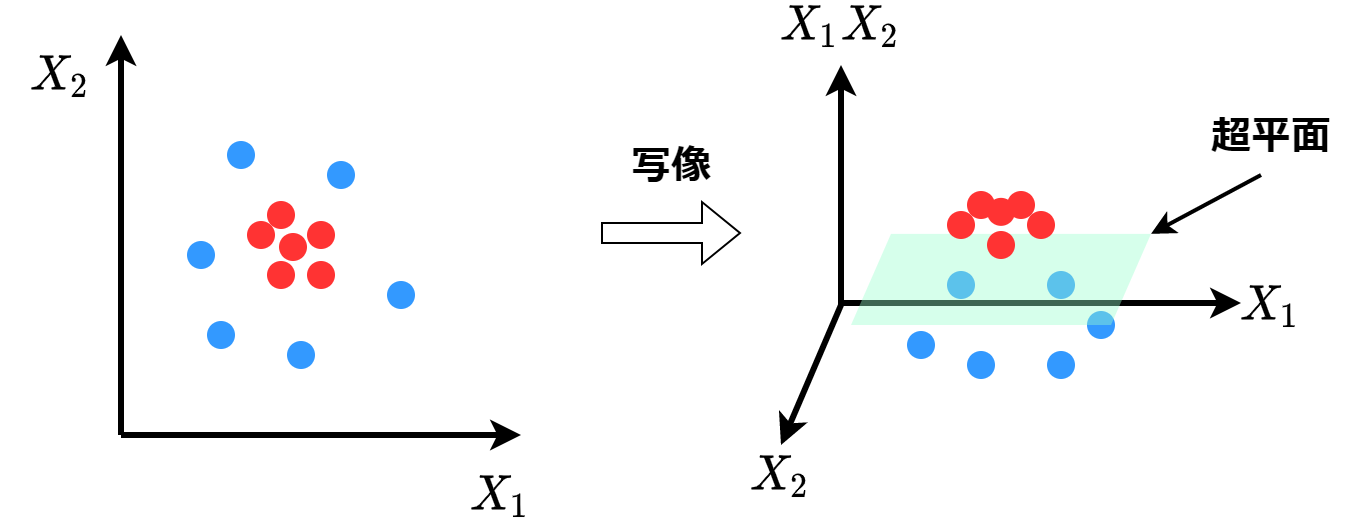
\includegraphics[width=0.8\linewidth]{syazou.png}
    \caption{高次元空間への写像の例}
    \label{syazou}
\end{figure}
一般に,線形分離可能性はデータのサンプル数が多くなればなるほど難しくなり,
特徴空間の次元数が大きくなるほど易しくなる.特に,$n-1$次元空間では,
最大で$n$個のデータを任意のラベル付けで線形分離可能である.
そのため$N$次元特徴ベクトルを$N^{\prime} $次元特徴空間に写像することで線形分離可能性が向上する.
ここで,$N$次元特徴ベクトルを$N^{\prime} $次元特徴空間に写像する関数を
$\boldsymbol{\phi}(\boldsymbol{x}) = \{\phi_i(\boldsymbol{x}),...,\phi_{N^{\prime}}(\boldsymbol{x})\}^T$
とすると,特徴空間上での分離超平面は(\ref{feature1}),(\ref{feature2})式の最適化問題を解くことで得られる.
\begin{subequations}
\begin{align}  
    \underset{\boldsymbol{a}}{\text{max}} \left\{\tilde{L}(\boldsymbol{\alpha}) 
    = \sum_{i=1}^{n}\alpha_i - \dfrac{1}{2}\sum_{i,j=1}^{n}\label{feature1}
    \alpha_i\alpha_j y_i y_j \boldsymbol{\phi}(\boldsymbol{x_i})^T \boldsymbol{\phi}(\boldsymbol{x_j})\right\}  \\
    \text{subject to} \sum_{i=1}^{n}\alpha_i y_i = 0,0 \leq \alpha_i \leq C,\ (i=1,...,n)\label{feature2}
\end{align}
\end{subequations}
しかし次元$N^{\prime}$が大きくなればなるほど
$\boldsymbol{\phi}(\boldsymbol{x_i})^T \boldsymbol{\phi}(\boldsymbol{x_j})$
の計算量が膨大になる.
そこでカーネル関数を(\ref{karnel})式で定義する.
\begin{align}
    \label{karnel}
  K( \boldsymbol{x_i}, \boldsymbol{x_j}) = \boldsymbol{\phi}(\boldsymbol{x_i})^T \boldsymbol{\phi}(\boldsymbol{x_j})
\end{align}
もし,(\ref{karnel})式を満たすようなカーネル関数が存在するならば,入力特徴ベクトルの内積計算で
$\boldsymbol{\phi}(\boldsymbol{x})$
を得ることができる.すなわち計算量が膨大になる可能性がある
$\boldsymbol{\phi}(\boldsymbol{x_i})^T \boldsymbol{\phi}(\boldsymbol{x_j})$
を直接計算する必要がない.このように内積計算をカーネル関数で置き換える手法をカーネルトリックと呼ぶ.
本実験では,(\ref{k1})〜(\ref{k4})式で表されるカーネル関数をハイパーパラメータの対象とする.
また,(\ref{k1})〜(\ref{k4})式内にあるハイパーパラメータは$\gamma$,coef0,$d$の3つである.
\begin{align}
    \text{線形カーネル:} \quad K(\boldsymbol{x_i}, \boldsymbol{x_j}) &= \boldsymbol{x_i}^T \cdot \boldsymbol{x_j}\label{k1} \\
    \text{RBFカーネル:} \quad K(\boldsymbol{x_i}, \boldsymbol{x_j}) &= \exp\left(-\gamma \| \boldsymbol{x_i} - \boldsymbol{x_j} \|^2\right)\label{k2} \\
    \text{シグモイドカーネル:} \quad K(\boldsymbol{x_i}, \boldsymbol{x_j}) &= \tanh(\gamma \boldsymbol{x_i}^T \cdot \boldsymbol{x_j} + \text{coef0}) \label{k3}\\
    \text{多項式カーネル:} \quad K(\boldsymbol{x_i}, \boldsymbol{x_j}) &= (\gamma\boldsymbol{x_i}^T \cdot \boldsymbol{x_j} + \text{coef0})^d\label{k4}
\end{align}
%カーネル関数の条件を挙げるべきか(勉強不足)
\subsection{多クラス分類への拡張}
SVMは2値分類器であるが,1対他法や1対1法により多クラス分類への拡張ができる.
1対他法では,各クラスに対し,そのクラスとそれ以外のクラスの分類をする.
そのためクラスが$K$個ある場合,$K$個のSVMモデルを用意する必要がある.
一方,1対1法では各クラスのペアの組み合わせに対して分類をする.
そのためクラスが$K$個ある場合,$\frac{K(K-1)}{2}$個のSVMモデルを用意する必要がある.
以上より,より計算量が少ないのが1対他法,より詳細な分類をするのが1対1法の特徴である.
本研究では一対他法を使用する.

 % intro.tex を読み込む。
\clearpage
\section{ABCアルゴリズム}
\subsection{概要}
郡知能とは個々での単純な行動が,集団としては高度な振る舞いをすることを模した最適化アルゴリズムである.
ABCは2005年にkaraboraによって提案された郡知能の一つである[\cite{abc}].
ABCは蜜蜂の採餌行動から着想を得ており,収穫蜂,追従蜂,偵察蜂の3種類の蜂によって探索を行う.
収穫蜂はすべての食物源に対して探索を行い,追従蜂は評価値の高い食物源を優先して探索を行なう.
追従蜂の探索によって評価値の高い食物源の近傍を局所的に探索することができる.
収穫蜂と追従蜂による探索で改善されなかった食物源は偵察蜂によってランダムな新しい食物源に置き換えられる.
偵察蜂によって局所最適解からの脱出が可能になり,探索範囲を広げることができる.
これら3種類の蜂による探索を繰り返すことで,より良い解を求めていく.
\subsection{探索手順}
ABCによって,(\ref{problem})式のような目的関数を$f(x)$を最小とするD次元の$x$を求める問題を解くことを考える.
\begin{align}
    \label{problem}
\text{min}.f(x), \text{~~subject to } \boldsymbol{x} \in \mathbb{R} ^D
\end{align}
ABCでは食物源の数$n$と探索上限回数$limit$の2つのパラメータをあらかじめ設定する必要がある.
食物源の数を$n$とすると,収穫蜂,追従蜂の数はそれぞれ$n$ずつとなる.
$limit$は偵察バチフェーズで使用する食物源の探索回数の上限である.
この値を小さくするとより広範囲の探索に,大きくするとより局所的な探索を行う.
各食物源に番号を振り分け,$i$番目の食物源を$\boldsymbol{x_{i}}(i = 1,...,n)$とすると
$\boldsymbol{x_{i}}$の評価値$fit(\boldsymbol{x_{i}})$は
(\ref{eva})式の評価関数により求められる.
\begin{align}
    \label{eva} 
    fit(\boldsymbol{x_{i}}) =
    \begin{cases}
    \dfrac{1}{1+f(\boldsymbol{x_{i}})} & \text{if } f(\boldsymbol{x_{i}}) \geq 0   \\
    \left\lvert1+f(\boldsymbol{x_{i}})\right\rvert & otherwise
    \end{cases}
\end{align}
\subsubsection*{step 0 準備}
ABCにおけるパラメータである食物源の数$n$と探索上限回数$limit$の設定を行う.次に終了条件の設定を行なう.
終了条件としては,アルゴリズムの反復回数が最大反復回数を超えたとき,
最良の食物源の評価値もしくは目的関数値が一定値を超えたときなどがある.
\subsubsection*{step 1 初期化}
初期化では,(\ref{init})式によって各食物源を各成分の範囲内でランダムに生成する.
さらに各食物源の探索回数$trial_i$を0に初期化する.
$x_{ij}$は$\boldsymbol{x_{i}}$,の$j(j=1,...,D)$番目の成分, 
$xmin_j$, $xmax_j$はそれぞれ食物源の各成分の最小値,最大値である.また,$rand$は一様乱数を表す. 
\begin{align}
    x_{ij} = xmin_j + rand[0,1](xmax_j-xmin_j)\label{init}
\end{align}
初期化された食物源の中で最も評価値が高いものを$\boldsymbol{x}_{best}$とし,
その食物源のインデックスを$i_{best}$とする
\subsubsection*{step 2 収穫蜂フェーズ}
収穫蜂フェーズでは収穫蜂が食物源の近傍を探索する.
このときの更新式は(\ref{harvest})式のようになる.
ここで$j,k(k\neq i)$はランダムに選択される.
\begin{align}
v_{ij} = x_{ij} + rand[-1,1](x_{ij}-x_{kj})\label{harvest}
\end{align}
ここで$v_{ij}$と$x_{ij}$の評価値を比較し, $v_{ij}$が$x_{ij}$よりも優れていたら$x_{ij}$を$v_{ij}$に置き換え,
$trial_i$を0にリセットする.
そうでなければ,$trial_i$を1増やす.
\subsubsection*{step 3 追従蜂フェーズ}
追従蜂フェーズでは収穫蜂フェーズによって更新された食物源の評価値に基づいて,
ルーレット選択を行い更新個体を選択する.
食物源$x_i$の選択確率$p_i$は(\ref{roulette})式のようになる.
そのため,評価値が高い食物源ほど選択確率が高く,評価値が低い食物源は選択確率が低くなる.
食物源の更新は収穫蜂フェーズと同様に行われる.
この操作を$n$回行う.
\begin{align}
    p_i = \dfrac{fit(\boldsymbol{x_{i}})}{\sum_{n}fit_j}\label{roulette}
\end{align}
\subsubsection*{step 4 偵察蜂フェーズ}
偵察蜂フェーズでは,$trial$の値が探索打ち切り回数$limit$に達した
食物源を(\ref{init})式によりランダムに生成した新たな解に置換する. 
置換した食物源の$trial$を0にリセットする.
$trial$の値が$limit$に達した
食物源がなければ何も行わない.
\subsubsection*{step 5 終了判定}
各食物源の評価値$fit(\boldsymbol{x_{i}})$と,$fit(\boldsymbol{x}_{best})$を比較し,
$fit(\boldsymbol{x_{i}}) > fit(\boldsymbol{x}_{best})$となる$\boldsymbol{x_{i}}$が存在する場合は
$\boldsymbol{x}_{best}$を更新する.
その後,終了条件を満たしている場合は最適解をその時の$\boldsymbol{x}_{best}$として探索を終了し,
そうでない場合は\textbf{step 2}に戻り,探索を続ける.
 % intro.tex を読み込む。
\clearpage
\section{提案手法}
先行研究では,カーネル関数をrbfに固定してハイパーパラメータ最適化を行っていた.
しかし,
本研究では,SVMのハイパーパラメータ$C$に加え,
(\ref{k1})〜(\ref{k4})式の4つのカーネル関数とそのハイパーパラメータ($\gamma$,coef0,$d$)
を最適化対象とする手法を提案する.
最適化アルゴリズムは設定パラメータの少ないABCを使用する.
これにより,ハイパーパラメータの探索範囲を広げ,より良いSVMモデルの探索が可能になる.
\subsection{ABCアルゴリズムの適用}
(\ref{k1})〜(\ref{k4})式の4つのカーネル関数は,ハイパーパラメータの数や性質が異なっている.
そのためカーネル関数が異なる個体では個体表現が変わり,個体の次元数が変化する.
しかし,(\ref{k2})〜(\ref{k4})式の$\gamma$や,
(\ref{k3}),(\ref{k4})式のcoef0はそれぞれスケール項,定数項と共通の性質を持っている.
そこで,本研究ではABCの個体表現を(\ref{expression})の5次元とし,
個体表現の変化をその個体の各次元の活性,非活性により表現することとした.
ここで,カーネル関数,$C$は常に使用されるハイパーパラメータで
$\gamma$,coef0,$d$はその個体のカーネル関数によって活性,非活性になる.
\begin{align}
    \text{個体表現:} \quad  (\text{カーネル関数},~C,~\gamma,~\text{coef0},~d)\label{expression}
\end{align}
$C,~\gamma,~\text{coef0},~d$は[0.1]の範囲の実数とし,(\ref{map})式によって
SVMに適用される値に変換される.
カーネル関数の値は4つのカーネル関数を整数値にエンコードしたものである.
また,$d$は離散値であるため,$A$を四捨五入したものをSVMに適用し,非活性の次元は探索の際に選択されない.
表~\ref{tab:param}にカーネル関数による活性,非活性の状態の組み合わせを示す.ここで1が活性,0が非活性を表す.
\begin{table}[t]
    \centering
    \caption{カーネル関数によるパラメータの活性,非活性}  % 表のキャプション
    \begin{tabular}{|c|c|c|c|}  % 3列を定義(c: 中央揃え,|: 縦線)
        \hline  % 横線
        カーネル関数 & $\gamma$ & coef0 & $d$\\  % ヘッダー行
        \hline  % 横線
        線形カーネル& 0& 0& 0\\  % 1行目
        \hline  % 横線
        RBFカーネル & 1 & 0& 0\\  % 2行目
        \hline  % 横線
        シグモイドカーネル & 1 & 1& 0\\  % 2行目
        \hline  % 横線
        多項式カーネル & 1 & 1& 1\\  % 2行目
        \hline  % 横線
    \end{tabular}
    
    \label{tab:param}  % 表のラベル
  \end{table} % 表のラベル
  
また,ABCによる最適化は連続値を前提としているため,
カテゴリ変数であるカーネル関数にABCの更新式は適用できない.
そこで本研究では更新次元にカーネル関数が選択された際の更新は
(\ref{karnel_update})式の確率$P$で更新されるものとする.
ここで$\boldsymbol{x_i}$は更新個体,
$\boldsymbol{x_j}$は$\boldsymbol{x_i}$と異なるカーネル関数を持つ個体の中からランダムに選ばれた個体である.
\begin{align}
    \label{karnel_update}
   P = \dfrac{f(\boldsymbol{x_j})}{f(\boldsymbol{x_i})+f(\boldsymbol{x_j})}
\end{align}
ABCにおける食物源の評価値は(\ref{fitness})式によって計算される.
\subsection{提案手法のアルゴリズム}
図~\ref{flowchart}にABCアルゴリズムによる最適化手順を示す.
\begin{figure}
    \centering
    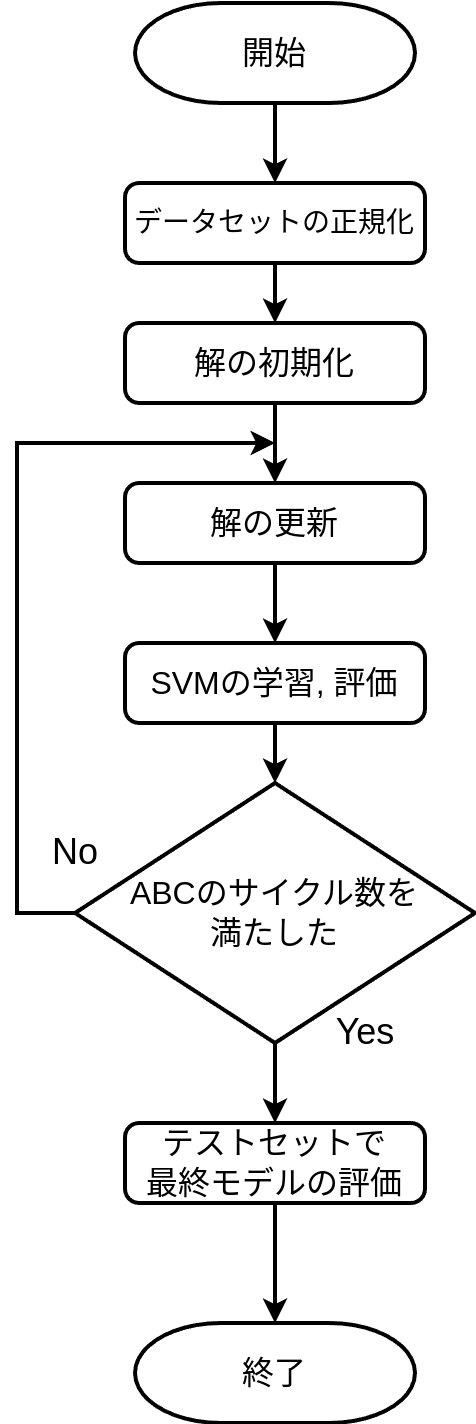
\includegraphics[width=0.4\linewidth]{flowchart.png}
    \caption{提案手法の最適化手順} 
    \label{flowchart}
\end{figure}
ABCアルゴリズムの詳細な手順を以下に示す.
ただし評価値の計算は次の手順で行われる.
\begin{enumerate}
    \item カーネル関数以外の値を(\ref{map})式でマッピング.
    \item その食物源が多項式カーネルだった場合$d$の値を四捨五入.
    \item 学習セットでsvmの学習を行う.
    \item 検証セットでsvmの分類精度を算出.
    \item (\ref{fitness})式で評価値の計算
\end{enumerate}

\subsubsection*{step 0 準備}
ABCにおけるパラメータである食物源の数$n$と探索上限回数limitの設定を行う.
次にSVNのハイパーパラメータ$C$,$\gamma$,coef0,$d$の探索範囲の設定を行い,
4つのカーネル関数を整数値にエンコードする.
最後に終了条件であるアルゴリズムのサイクル数を設定する.
\subsubsection*{step 1 初期化}
初期化では,$n$個の食物源をカーネル関数を定める1次元目を1〜4の整数値でランダムに初期化,
その他の2〜5次元は[0,1]の一様乱数で初期化する.
$n$個の食物源の評価値を計算し,
初期化された食物源の中で最も評価値が高い食物源
とそのインデックスを保存する.
\subsubsection*{step 2 収穫蜂フェーズ}
収穫蜂フェーズでは収穫蜂が食物源の近傍を探索する.
このときの更新式は(\ref{harvest})式のようになる.
ここで$j,k(k\neq i)$はランダムに選択される.
\begin{align}
v_{ij} = x_{ij} + \,mathrm{rand}[-1,1](x_{ij}-x_{kj})
\end{align}
ここで$v_{ij}$と$x_{ij}$の評価値を比較し,$v_{ij}$が$x_{ij}$よりも優れていたら$x_{ij}$を$v_{ij}$に置き換え,
$trial_i$を0にリセットする.
そうでなければ,$trial_i$を1増やす.
\subsubsection*{step 3 追従蜂フェーズ}
追従蜂フェーズでは収穫蜂フェーズによって更新された食物源の評価値に基づいて,
ルーレット選択を行い更新個体を選択する.
食物源$x_i$の選択確率$p_i$は(\ref{roulette})式のようになる.
そのため,評価値が高い食物源ほど選択確率が高く,評価値が低い食物源は選択確率が低くなる.
食物源の更新は収穫蜂フェーズと同様に行われる.
この操作を$n$回行う.
\begin{align}
    p_i = \dfrac{\mathrm{fit}(\boldsymbol{x_{i}})}{\sum_{n}\mathrm{fit}(\boldsymbol{x_{j}})}
\end{align}
%\subsubsection*{step 3 追従蜂フェーズ}
%追従蜂フェーズでは評価回数を減らすためにルーレット選択とは異なる手法に変更している.
%各食物源$x_i$に対して1回ずつの更新確率$1 - p_i$で食物源の更新を行う.
%食物源の更新は収穫蜂フェーズと同様に行われる.
%確率未満の食料源は無視される.
%この操作を$n$回行う.
%そのため追従蜂の数は0〜nでランダムである.
\subsubsection*{step 4 偵察蜂フェーズ}
偵察蜂フェーズでは,trialの値が探索打ち切り回数limitに達した
食物源をstep 1 の初期化と同じ手順でランダムな新たな解に置換する. 
置換した食物源のtrialを0にリセットする.
trialの値がlimitに達した
食物源がなければ何も行わない.
\subsubsection*{step 5 終了判定}
各食物源の評価値と,この時点で最良の食物源の評価値を比較し,
$\mathrm{fit}(\boldsymbol{x_{i}}) > \mathrm{fit}(\boldsymbol{x}_{best})$となる$\boldsymbol{x_{i}}$が存在する場合は
$\boldsymbol{x}_{best}$を更新する.
その後,指定したサイクル数を満たしていない場合は\textbf{step 2}に戻り,探索を続ける.
指定したサイクル数に達していた場合は,最適解をその時の$\boldsymbol{x}_{best}$として探索を終了し,
$\boldsymbol{x}_{best}$を適用したSVMモデルのテストセットに対する分類精度を算出する. % intro.tex を読み込む。
\clearpage
\section{実験}
侵入検知問題である10\%KDD'99データセットを使用して,
scikit-learnのデフォルトパラメータ,既存手法,提案手法の間で表~\ref{tab:1}の設定で比較実験を行った.
実験は,データセットからランダムに10\%抽出した学習セット,検証セット,テストセットの3つのデータセットを用意して行った.
検証セットはABCアルゴリズムにおける解の評価に使われ,
得られた最適解を未知のデータであるテストセットの分類に適用し
,その結果を最終的な分類精度とする.
\subsection{データセット}
10\%KDD'99データセットは,オリジナルのKDD'99データセットのうちサンプル数の多いnormal,
dos,probeクラスを10\%に減らしたデータセットである.また,KDD'99データセットの特徴数は41個である.
KDD'99データセットの内訳を表~\ref{kdd99}に示す.
\begin{table}[tb]
    \centering
    \begin{minipage}{0.45\textwidth}  % 表の幅を指定
        \centering
        \caption{KDD'99データセットの内訳}  % 表のキャプション
        \begin{tabular}{|l|r|r|}  % 左揃えと右揃えに変更
          \hline  % 横線
          クラス & KDD'99 & 10\%KDD'99 \\  % ヘッダー行
          \hline  % 横線
          normal & 972780 & 97279 \\  % 1行目
          \hline  % 横線
          dos & 3883370 & 391458 \\  % 2行目
          \hline  % 横線
          probe & 41102 & 4107 \\  % 3行目
          \hline  % 横線
          r2l & 1126 & 1126 \\  % 4行目
          \hline  % 横線
          u2r & 52 & 52 \\  % 5行目
          \hline  % 横線
          合計 & 4898430 & 494021 \\  % 合計行
          \hline  % 横線
        \end{tabular}
        \label{kdd99}  % 表のラベル 
    \end{minipage}
    \begin{minipage}{0.45\textwidth}  % 表の幅を指定
        \centering
        \caption{実験データセットの内訳}  % 表のキャプション
        \begin{tabular}{|c|c|c|c|}  % 列を定義
          \hline  % 横線
          クラス & 学習 & 検証 & テスト \\  % ヘッダー行
          \hline  % 横線
          normal & 9740 & 9650 & 9766 \\  % 1行目
          \hline  % 横線
          dos & 39127 & 39238 & 39106 \\  % 2行目
          \hline  % 横線
          probe & 412 & 385 & 410 \\  % 3行目
          \hline  % 横線
          r2l & 120 & 125 & 115 \\  % 4行目
          \hline  % 横線
          u2r & 3 & 4 & 5 \\  % 5行目
          \hline  % 横線
          合計 & 49402 & 49402 & 49402 \\  % 合計行
          \hline  % 横線
        \end{tabular}
        \label{3kdd99}  % 表のラベル 
    \end{minipage}
  \end{table}
本研究では,ABCで得られたSVMモデルが未知のデータに対して有効であるかを評価するために
3つのデータセットを用意した\cite{origin}.3つのデータセットは,
SVMの学習に使用する学習セット,SVMの評価に使用する検証セット,
最適解を評価するためのテストセットである.
ここでテストセットはABCで得られた最適解を評価するために一度だけ使用される.
3つのデータセットを内訳を表~\ref{3kdd99}に示す.
これらのデータセットは10\%KDD'99データセットからランダムに10\%抽出している.
\subsection{実験設定}
\subsubsection{実験環境}
SVMの実装には,CPU:Intel Core i7-12700,メモリ32GBの計算機上で
Python~3.11.0とscikit-learn~1.5.0ライブラリのSVCクラスを使用した.
SVCクラスにおける本研究で使用するハイパーパラメータのデフォルト設定を表~\ref{default}に示す.
ここでn\_featureはデータセットの特徴数を表す.
\begin{table}[tb]
    \centering
    \caption{SVCクラスのデフォルト設定}
    \begin{tabular}{|c|c|}  % 2列を定義
      \hline  % 横線
      パラメータ & デフォルト値 \\  % ヘッダー行    
      \hline  % 横線
      kernel & rbf\\  % 2行目
      \hline  % 横線
      $C$ & 1.0 \\  % 1行目
      \hline  % 横線     
      $\gamma$ & 1/n\_feature\\  % 3行目
      \hline  % 横線
      coef0 & 0\\  % 4行目
      \hline  % 横線
      degree($d$) & 3\\  % 4行目
      \hline  % 横線
  \end{tabular}
     % 表のキャプション
    \label{default}  % 表のラベル 
  \end{table}
\subsubsection{パラメータ設定}
表~\ref{abc:param},\ref{svm:param}に本研究のパラメータ設定を示す
\begin{table}[tb]
    \centering
    \begin{minipage}{0.45\textwidth}  % 左側の表の幅
      \centering
      \caption{ABCの実験パラメータ}  % 表のキャプション
      \begin{tabular}{|c|c|}  % 2列を定義
        \hline  % 横線
        コロニーサイズ & 20 \\  % ヘッダー行
        \hline  % 横線
        LIMIT & 100 \\  % 1行目
        \hline  % 横線
        サイクル数 & 500 \\  % 2行目
        \hline  % 横線
      \end{tabular}
      \label{abc:param}  % 表のラベル 
    \end{minipage}
    \begin{minipage}{0.45\textwidth}  % 右側の表の幅
      \centering
      \caption{SVMの実験パラメータ}  % 表のキャプション
      \begin{tabular}{|c|c|}  % 2列を定義
        \hline  % 横線
        kernel & [linear,rbf,sigmoid,poly] \\  % 2行目
        \hline  % 横線
        $C$ & [$10^{-6}$,35000] \\  % 1行目
        \hline  % 横線     
        $\gamma$ & [$10^{-6}$,32] \\  % 3行目
        \hline  % 横線
        coef0 & [0,10] \\  % 4行目
        \hline  % 横線
        degree($d$) & [1,3] \\  % 4行目
        \hline  % 横線
      \end{tabular}
      \label{svm:param}  % 表のラベル 
    \end{minipage}
  \end{table}
\subsection{実験結果}
実験結果を表~\ref{result}に示す.
\begin{table}[h]
    \centering
    \caption{実験結果}  % 表のキャプション
    \begin{tabular}{|c|c|c|c|c|c|c|}  % 3列を定義(c: 中央揃え、|: 縦線)
        \hline  % 横線
        ~ & 線形 &rbf &シグモイド&多項式&既存手法 & 提案手法\\  % ヘッダー行
        \hline  % 横線
        分類精度[\%]& 99.68&99.78&96.12&99.76&99.84& 99.90\\  % 1行目
        \hline  % 横線
        実行時間[h] & - & -&-&-&11.7& 7.0\\  % 2行目
        \hline  % 横線
    \end{tabular}
   
    \label{result}  % 表のラベル
  \end{table} % intro.tex を読み込む。
\clearpage
\section{考察}
内容1

\clearpage
\section{おわりに}
本研究では,カーネル関数を含むハイパーパラメータ全体を探索対象とし,
ABCアルゴリズムを用いてSVMのハイパーパラメータ最適化を行う手法を提案した.
ABCアルゴリズムでカーネル関数を扱うために新たな更新式と探索アルゴリズムを導入した.
実験はKDD'99データセットを学習セット,検証セット,テストセットの3つに分けて
使用し,SVCクラスのデフォルトパラメータ,先行研究,提案手法の間で比較実験を行った.
その結果,提案手法の実行時間は先行研究よりも長くなってしまったが,
分類精度の面で先行研究よりも良い結果を得ることができた.
また,検知率,誤警報率,適合率,F値の値も改善することができ,
侵入検知問題への性能も向上した.
このことから,提案手法は実行時間よりも
モデルの性能を重視する環境において有用であると言える.

今後の課題としては, KDD'99データセット以外のデータセットでも実験を行うことや
先行研究よりも長くなってしまった実行時間の短縮を図ることが挙げられる.
特にその他のデータセットでも実験を行うことは重要で,
提案手法はカーネル関数もハイパーパラメータとして扱ったため,
様々なデータセットにおいても良い性能を発揮することが期待できる.

本研究で扱ったKDD'99データセットは比較的大規模なデータセットであるため,
SVMの学習を打ち切ったり,多項式カーネルの次元数の探索範囲を低く設定したが,
小規模なデータセットにおいてはこれらの制約を設けることなくハイパーパラメータの最適化
ができると考えられる.





 % intro.tex を読み込む。
\clearpage

\謝辞 % ここから謝辞
山口先生有り難う! % 謝辞のないよう
\clearpage

\begin{thebibliography}{99} % 参考文献をここに書く(TeXの参考書を参照)
\addcontentsline{toc}{section}{参考文献}
\bibitem{essential}M. Feurer and F. Hutter, “Hyperparameter optimization,” Automated Machine Learning, pp.3–33, Springer, 2019.
\bibitem{origin}近藤 久,浅沼 由馬“人工蜂コロニーアルゴリズムによるランダムフォレストとサポートベクトルマシンのハイパーパラメータ最適化と特徴選択”,
人工知能学会論文誌, vol34-2, pp.1-11, 2019.
\bibitem{svm}Cortes, C. and Vapnik, V. Support-vector networks, Ma-chine Learning, Vol.20, No.3, pp.273-297, 1995.
\bibitem{abc}Karaboga, Dervis. An idea based on honey bee swarm for numerical optimization. Vol. 200. 
Technical report-tr06, Erciyes university, engineering faculty, computer engineering department, 2005.
\end{thebibliography} % 参考文献環境の終了
\end{document} % 本文の終了
